%
%  Vorlage/Template fuer #EBT
%
%  Created by Prof. Dr. Detlef Kreuz on 2010-08-14.
%  Copyright (c) 2010 . All rights reserved.
%
\documentclass[12pt,toc=bib,toc=listof]{scrreprt}
\usepackage[ngerman]{babel} 
\usepackage[utf8]{inputenc}
\usepackage[T1]{fontenc}
\usepackage{lmodern}
\usepackage{setspace}
\usepackage{listings}
\usepackage{enumitem}


\usepackage{hyperref}
\hypersetup{
  ,colorlinks=true
  ,linkcolor=blue
  ,citecolor=blue
  ,filecolor=blue
  ,urlcolor=blue
  }

%%%%%%%%%%%%%%%%%%%%%%%%%%%%%%%%%%%%% % (fold)
% Vom Studierenden zu aendernde Werte
\newcommand{\ebttopic}{Docker}
\newcommand{\ebtstudentname}{Jerome Tagliaferri}
\newcommand{\ebtstudentid}{190530}
\urldef{\ebtstudentmail}\url{jtagliaf@stud.hs-heilbronn.de}
%
%%%%%%%%%%%%%%%%%%%%%%%%%%%%%%%%%%%%% % (end)

\usepackage{ifpdf}
\ifpdf
\usepackage[pdftex]{graphicx}
\else
\usepackage{graphicx}
\fi

\graphicspath{{images/}}
\usepackage[headsepline]{scrpage2}
\pagestyle{scrheadings}
\clearscrheadfoot
\ihead{Fallstudie Entwicklungswerkzeuge: \ebttopic}
\ohead{\pagemark}
\renewcommand*{\chapterpagestyle}{scrheadings}
\renewcommand*{\chapterheadstartvskip}{}

\titlehead{\flushright
%\includegraphics{HHN_KOMPLETT_4C.jpg}

\includegraphics[scale=0.6]{HHN_ab_40_mm_4c_neg.png}
}
\subject{Fallstudie Entwicklungswerkzeuge (281761)}
\title{\ebttopic}
\author{\ebtstudentname\footnote{\ebtstudentid, \ebtstudentmail}}
%% Datum nie auf einen festen Wert setzen
\publishers{Eingereicht bei Paul Lajer}

%\pagestyle{headings}

\begin{document}
\pagenumbering{roman} 
\selectlanguage{ngerman}
\maketitle
\tableofcontents


% chapter abkuerzungsverzeichnis (end)

\listoffigures

\onehalfspacing
\newpage
\pagenumbering{arabic}

\chapter{Einleitung} % (fold)
\label{sec:einleitung}

\section{Motivation} % (fold)
\label{sec:motivation}

In einer extrem kompetitiven wirtschaftlichen Umgebung, welche sich durch die Weiterentwicklung von technischen Systemen immer schneller und vor allem grundlegend verändert,
ist es notwendig, seine Dienste auf einer flexiblen und skalierbaren Basis zu betreiben.\\
\\
Auf diesem Hintergrund, sind viele Technologien im Big Data und Cloud Umfeld entstanden und gewachsen.
Allen voran die Virtualisierung von Ressourcen und Systemen als Grundlage des Cloud Computing, mit dem Ziel auf individuelle Wünsche und eine stetig schwankende Ressourcenverteilung zu reagieren.
So wie diese Technologie ihren Weg in viele weitere Bereiche geebnet hat, findet die Container Virtualisierung eine immer vielseitigere und intensivere Anwendung.
Getragen und weiterentwickelt von Branchengrößen wie Google oder IBM ist die Container Virtualisierung momentan eine der sich am schnellsten wachsenden Bereiche der Informatik welche eine noch stärkere Flexibilität und Automatisierung von Systemen und Ressourcen verspricht.\\
\\
Aus diesem Grund, stellt die Container Virtualisierung ein relevantes Thema für jede Branche dar, welche mit Soft- und Hardwaresystemen in Kontakt kommt um in einem stetig veränderten Markt zu bestehen.


% section motivation (end)

\section{Ziel der Arbeit} % (fold)
\label{sec:ziel_der_arbeit}

Diese Ausarbeitung soll als Einstieg in den Bereich Container Virtualisierung dienen und dabei Docker als zentrale Komponente behandeln und vorstellen.\\
\\
Es soll ein umfassender Einblick in die Thematik und deren unterschiedliche Herangehensweisen erörtert werden, wodurch eingeschätzt werden kann, inwieweit sich die Container Virtualisierung für individuelle Einsatzzwecke eignet.
Dabei werden Anregungen für weitere Tools und Systeme gegeben welche diese Funktionalitäten erweitern und teilweise automatisieren. 

% section ziel_der_arbeit (end)

\section{Vorgehensweise} % (fold)
\label{sec:vorgehensweise}

Um dieses Ziel zu erreichen, werden die Grundlagen in Form der Idee und grundlegenden Historie und deren Konzepte, welche die Basis von Docker darstellen, erläutert.
Weiter wird die Umsetzung dieser Konzepte und deren Erweiterungen betrachtet und auf Basis eines einfachen Anwendungsbeispieles erläutert.
Anschließend werden die Ergebnisse gebündelt und in Vor- und mögliche Nachteile unterteilt.\\
\\
Aufbauend auf diesen Grundlagen werden Anwendungsbereiche vorgestellt, in denen Docker in einem produktiven Umfeld eingesetzt wird und welche Tools den massiven und verteilten Einsatz von Containern erleichtern.
Mögliche Alternativen und deren Unterschiede, sowie ein Ausblick in die Zukunft der Container Virtualisierung, sollen diese Arbeit abschließen.



% section vorgehensweise (end)
% chapter einleitung (end)

\chapter{Docker Grundlagen} % (fold)
\label{sec:grundlagen}

\section{Definition}

Die Bezeichnung Docker findet schon lange nicht nur im Cloud spezifischen Umfeld Erwähnung.
Der aufmerksame Nutzer stößt immer öfter schon bei der Installation von Anwendungen auf diesen Term.\\
\\
Ein Beispiel hierfür wäre das Test und Entwicklungswerkzeug Jenkins, welches nun an erster Stelle die Option eines Docker Containers, als mögliche Installationsquelle, zur Verfügung stellt. \cite{jenkins}
Viele weitere Hersteller, welche Werkzeuge anbieten und auf unterschiedlichste Bibliotheken und Dienste angewiesen sind, greifen immer öfter zu Docker. 
Hierbei stellt sich jedoch die Frage: „Was ist Docker?“ \\
\\
Auf der Offiziellen Seite wird diese Frage mit folgendem Satz beantwortet :

\begin{quote}
	\footnote[1]{Vgl. https://www.docker.com/what-docker}
	"`\textit{Docker is the world's leading software containerization platform}"
\end{quote}
Da diese Aussage wenig bis keinen Informationsgehalt bietet, macht es Sinn, sich zuerst einmal die grundlegenden Konzepte und historische Entwicklung der Container Virtualisierung anzuschauen. 

\section{Konzepte und Entwicklungsgeschichte}

Wie so viele Entwicklungen im technischen Umfeld sind die Konzepte und ersten Umsetzungen der Container Virtualisierung schon weitaus älter.\\
\\
Hierbei tauchten erste Ansätze, welche später den Grundstein darstellen sollten, schon 1979 auf.
Es begann dabei alles mit der Idee Services untereinander und vom eigentlichen Host System isolieren zu können.\\
\\
Dieses Konzept wurde erstmals unter UNIX in der Form des "chroot" umgesetzt.
Diese Funktion war in der Lage das Hauptverzeichnis eines Prozesses zu isolieren, indem ihm ein neuer Ort zugewiesen wurde. 
Erst im Jahre 2000 wurde diese Funktionalität unter FreeBSD mit dem Namen Jails erneut aufgenommen und erweitert.
Diesmal konnte nicht nur das Dateisystem isoliert werden, sondern auch dazugehörige Benutzer, Netzwerk und die zugehörigen Prozesse.
Über die nächsten acht Jahre entstanden somit viele weitere Technologien, welche diese Funktionalitäten integrierten. Darunter unter anderem der
Linux VServer, Oracle Solaris Zones, OpenVZ oder auch die von Google entwickelten Process Container.
Später wurde dann mit ControlGroups, ein weiterer wichtiger Baustein, Teil des Linux Kernels. 
Erst 2008 entstand dann, durch die Entwicklung bei IBM, das Linux Containers project (LXC) welches die unterschiedlichen Technologien, im Container Umfeld, zusammen brachte und somit die vollständigste Implementierung eines Linux Container Managements darstellte.
Die Besonderheit von LXC bestand darin, dass es seine Ressourcen komplett aus dem Linux Kernel bezog ohne dazu zusätzliche Software zu benötigen und somit den Einsatz enorm erleichterte.\\
\\
Am 15.03.2013 wurde Docker durch den dotCloud Gründer Solomon Hykes, zum ersten mal der Öffentlichkeit, in einem fünf minütigen Vortrag vorgestellt.
Diese Information traf jedoch einen Nerv, wodurch sich diese Ankündigung innerhalb kürzester Zeit weltweit verbreitete.
Dies hatte zur Folge, dass große Firmen, allen voran Google, großes Interesse an diesem Projekt verkündeten und es daraufhin auf GitHub offen gelegt wurde.


\section{Funktionsweise}

Abgesehen von der schnellen Verbreitung von Docker war vielen Interessenten die eigentliche Funktionsweise des Frameworks nicht vollständig bewusst.
Docker versprach, ein Stück Software in ein komplettes Dateisystem zu verpacken, welches alles beinhaltet was für das Ausführen dieser  nötig ist. 
Konkret bedeutet dies den Quellcode, System Bibliotheken und mögliche zusätzliche Dienste oder Middleware. 
Die Folge aus diesem vorgehen ist , dass sich die Software immer gleich verhält, egal auf welcher Umgebung sie ausgeführt wird. 
Hinzu kommt, das Container aufgrund ihrer Größe und Isolation  beliebig gestartet oder gestoppt werden können, ohne das Host System zu beeinflussen.\\
\\
Einige dieser Eigenschaften werden oftmals sehr gerne mit denen virtueller Maschinen verglichen, da es auf den ersten Blick sehr viele Ähnlichkeiten aufweist.
Die Entwickler von Docker distanzieren sich jedoch sehr klar von diesem Vergleich und machen darauf aufmerksam, dass Docker sehr viel mehr ist.
Docker hatte auch nie das bestreben danach, virtuelle Maschinen zu ersetzen, da beide Lösungen teils sehr unterschiedliche Anforderungen erfüllen sollen. 
Um jedoch die grundlegende Funktionsweise und Unterschiede zu erläutern, macht es Sinn diesen Vergleich zu bemühen.\\
\begin{figure}
	\centering
	\caption{VM vs Container}
	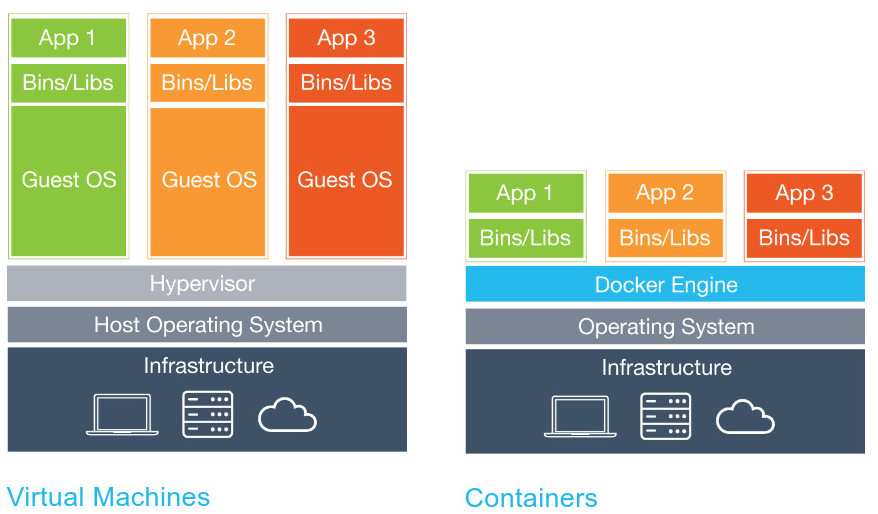
\includegraphics[width=15cm, height=8cm, scale=0.3]{dockerVM.jpg}
	Quelle: www.docker.com/what-docker
\end{figure}
\\
Wie in der Abbildung 2.1 zu erkennen, liegt ein sehr wesentlicher Unterschied in der Größe der Lösungsansätze, wie auch der Kommunikation zwischen Host-System und Client.
Da eine virtuelle Maschine über einen Hypervisor mit dem Host-System kommuniziert, bringt es bei jeder Instanz zusätzlich ein komplettes Gast Betriebssystem mit sich.
Dies führt zu einem erhöhten Ressourcenverbrauch, wodurch nur wenige Instanzen einer Virtuellen Maschine, auf einem Host System ausgeführt werden können.
Anwendungsbereiche in welchen eine noch stärkere Isolation aus Sicherheitsgründen notwendig ist, greifen deswegen genau aus diesem Grund auf VMs zurück.\\
\\
Docker wiederum kann über die Docker Engine direkt die Funktionen des Kernels nutzen und ist dadurch in der Lage mehrere hundert Container gleichzeitig zu betreiben.
Gerade hier verliert Docker jedoch an Sicherheit, da alle Applikationen auf denselben Kernel zurück greifen müssen.\\
\\
\\
\\
Damit dies möglich wird, greift Docker auf mehrere Funktionen des Linux Kernels zurück, welche in Abbildung 2.2 dargestellt sind.
Folgende zwei Funktionsweisen sind hierbei besonders wichtig:

\begin{itemize}
	\item \textbf{CGroups} : Limitiert und verwaltet die Ressourcen wie CPU , Arbeitsspeicher, Netzwerk und Festplattenzugriff, welche einer Prozessgruppe zugewiesen werden können. 
	\item \textbf{Namespace isolation} : Prozessgruppen sind nicht in der Lage die Ressourcen anderer Gruppen zu sehen.
\end{itemize}
\begin{figure}
	\centering
	\caption{Treiber}
	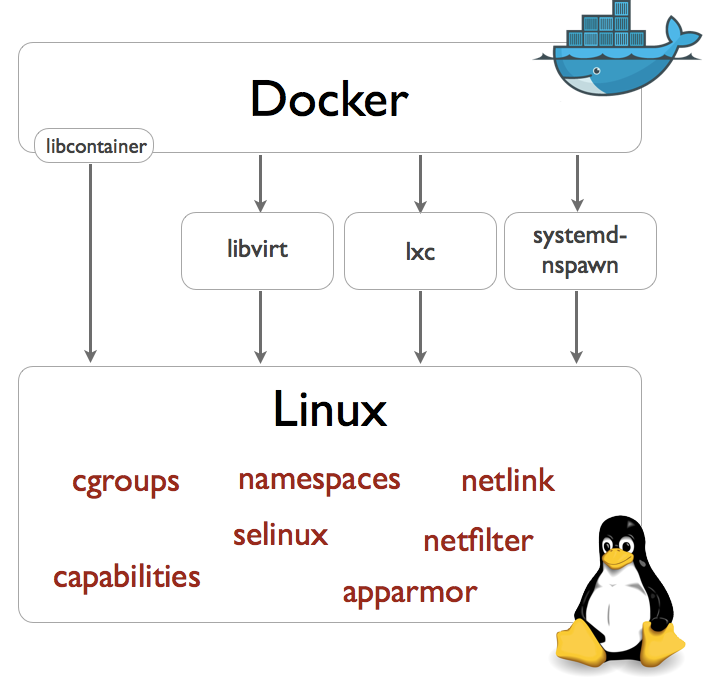
\includegraphics[width=13cm, height=9cm, scale=0.3]{docker-execdriver-diagram.png}\\
	Quelle: http://jancorg.github.io/blog/2015/01/03/libcontainer-overview
\end{figure}
Docker war lange Zeit noch von der LXC-Bibliothek abhängig, entwickelte jedoch parallel dazu eine eigene Lösung namens libcontainer, welche seit Version 0.9 standardmäsig verwendet wird. 
Diese neue Bibliothek wurde entwickelt um weitere Isolationstechniken zu nutzen und gleichzeitig in der Lage zu sein, alle zentralen Komponenten aus einer Hand liefern zu können.
Die Offenlegung dieser Funktion, gab auch Microsoft die Möglichkeit, Docker unter Windows zu unterstützen und öffnete die Tür für weitere Interessenten eigene Software in diesem Bereich zu entwickeln.\\
\\
Eine weitere sehr essentielle Komponente stellt UnionFS dar.
UnionFS ist ein Dateisystem, welches die Fähigkeit besitzt unterschiedliche Schichten (Standorte) von Dateien zu bündeln und anschließend einem Prozess zur Verfügung zu stellen.
Dies nutzt Docker, um nur neue oder veränderte Dateien dem Container Verfügbar zu machen.
Hierdurch kann die Geschwindigkeit in der Erstellung und dem Ausführen von Containern erheblich erhöht und beim Einsatz von großen mengen an Containern Speicherplatz gespart werden.


\section{Aufbau und Beispiel}

Aufbauend auf diesen Grundlagen, sollen nun die einzelnen Komponenten vorgestellt und danach an einem praktischen Beispiel angewandt werden.
Der Fokus soll dabei jedoch zuerst auf der Erstellung und Ausführung einer einzelnen Docker Instanz liegen.
Hierbei wurde auf eine Webapplikation zurück gegriffen, da diese meist auf unterschiedliche Bibliotheken und Services zurück greifen muss um vollständig einsatzfähig zu sein und somit den Einsatz von Containern optimal wiederspiegelen kann.\\
\\
Die wichtigsten Komponenten, für die Erstellung und Inbetriebnahme, sind wie folgt:
\begin{itemize}
	\item \textbf{Docker daemon}: Docker nutzt eine Client-Server Architektur wobei der Daemon einen serverseitigen Prozess darstellt, welcher die Aufgabe hat, Container zu erstellen, auszuführen und zu verteilen.
	\item \textbf{Docker CLI}: Der Docker Client hat die Möglichkeit, über eine REST API, mit dem Docker daemon zu kommunizieren und Befehle zu übermitteln.
	\item \textbf{Docker Image Index}: Ein öffentliches oder Privates Verzeichnis über alle Docker Images welche vorhanden sind. Möchte man ein Image ausführen, wird meist zuerst lokal nach solchem gesucht, sollte der Prozess nicht fündig geworden sein, wird im Docker eigenen Repository DockerHub weiter gesucht.
	\item \textbf{Docker Images}: Stellt ein Dateisystem mit verschiedenen Parametern dar, welches nur gelesen aber nicht beschrieben werden kann.
	\item \textbf{Dockerfiles}: Skripte welche den Bau eines Images vereinfachen und automatisieren.
	\item \textbf{Docker Containers}: Ein Container, welcher sich meist aus mehreren Images zusammen stellt. Diese enthalten alle nötigen Bibliotheken, Quellcode und Dienste um die Applikation auszuführen. Wenn ein solcher Container angelegt wird, wird wie in Abbildung 2.3 zu sehen ein neuer Layer angelegt, welcher Veränderungen aufnimmt und speichert.
\end{itemize}
\begin{figure}
	\centering
	\caption{Docker-Images}
	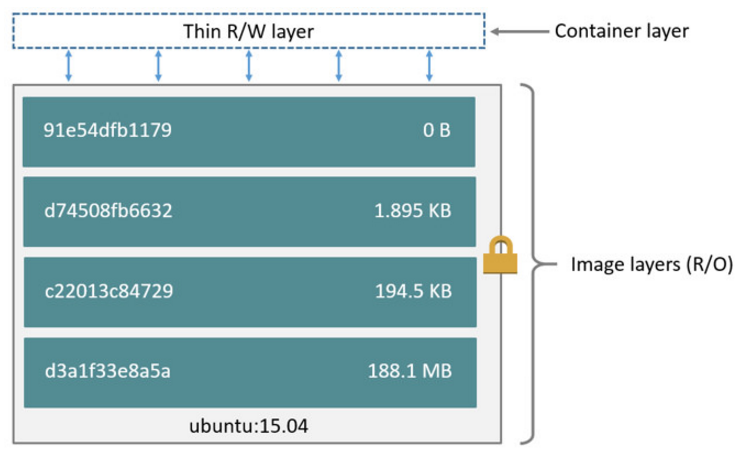
\includegraphics[width=15cm, height=8cm, scale=0.3]{container-images.png}
	Quelle: https://docs.docker.com/engine/userguide/storagedriver/imagesandcontainers/
\end{figure}
Das Zusammenspiel dieser Komponenten sorgt dafür, dass die Erstellung , Ausführung und Administration von Docker Containern schnell und einfach funktioniert.\\
\\
Die logische Abfolge dieser Komponenten soll nun anhand einer simplen Webapplikation verdeutlicht werden.
Wir gehen davon aus, dass Docker bereits auf dem Host System installiert wurde und eine  simple "Hello World !" Django Applikation angelegt ist.
Diese Applikation soll folgende Bibliotheken nutzen :\\
\\
\textit{Python 3}, \textit{Django 1.9.4} und \textit{Gunicorn 19.6} als Web Server.

\begin{enumerate}[leftmargin=*]
	
\item Um die Erstellung des Containers zu erleichtern, wird im Hauptverzeichnis der Applikation eine requirements.txt angelegt welche ausser Python alle benötigten Bibliotheken enthält. Die Dockerfile kann somit später auf diese Datei zugreifen und die benötigten Abhängigkeiten installieren. \\
In diesem Fall :

\noindent\hspace*{25pt}\textit{Django==1.9.4}\\
\noindent\hspace*{25pt}\textit{gunicorn==19.6.0}

\item Nun soll ein Skript erstellt werden, welches später die Ausführung des Gunicorn Web Servers, mit den gewünschten Parametern, übernehmen soll.
Hierzu wird eine start.sh Datei erstellt welche folgenden Inhalt besitzt :


\noindent\hspace*{25pt}\textit{ \#!/bin/bash\\
\noindent\hspace*{25pt}	exec gunicorn helloworld.wsgi:application \textbackslash \\
\noindent\hspace*{25pt}	-{}-bind 0.0.0.0:8000 \textbackslash \\
\noindent\hspace*{25pt}	-{}-workers 3 }

Über den exec Befehl wird  Gunicorn mit unserer helloworld Applikation gestartet, welche wir über die lokale Adresse 0.0.0.0 und den Port 8000 ansprechen wollen. Zur Sicherheit und verbesserten Bearbeitung von Anfragen werden zusätzlich drei Services (worker) erstellt.

\item Ab diesem Punkt, entsteht die eigentliche Arbeit mit Docker. 
Um dies zu bewerkstelligen, muss zuerst ein Dockerfile im Hauptverzeichnis der Anwendung erstellt werden.
Docker nutzt diese Datei später beim Bau des Containers wobei alle Befehle der Reihe nach abgearbeitet werden:

\noindent\hspace*{25pt}\textit{FROM python:3-onbuild\\
\noindent\hspace*{25pt}COPY . /usr/src\\
\noindent\hspace*{25pt}RUN pip install -r /requirements.txt
\noindent\hspace*{25pt}EXPOSE 8000\\
\noindent\hspace*{25pt}CMD ["usr/src/start.sh"]}

Hier eine kurze Erklärung der Befehle :
\begin{itemize}
	\item \textit{FROM}: Zieht sich ein Image aus dem lokalen oder externen DockerHub. In diesem Beispiel Python 3
	\item \textit{COPY}: Kopiert alle Dateien des momentanen Verzeichnisses an den definierten Ort im Container.
	\item \textit{RUN}: Führt den Befehl pip aus, welcher alle Bibliotheken die in der requirements.txt hinterlegt sind installiert.
	\item \textit{EXPOSE}: Öffnet den Port 8000 um später auf die Applikation zugreifen zu können.
	\item \textit{CMD}: Führt das Skript beim Start des Containers aus.
\end{itemize}

\item Über folgenden Befehl, wird über das Terminal die Dockerfile ausgeführt und ein Container mit dem Namen "'helloworld“ erstellt.

\textit{sudo docker build -t helloworld .}

\item Als letzter Schritt muss der Container nur noch  über das Terminal gestartet werden:

\textit{sudo docker run -it -p 8000:8000 helloworld}

Dies führt den Docker Container helloworld aus und reicht den Port 8000 des Host Systems, an den Port 8000 der Docker Instanz weiter.
\end{enumerate}
Steht dieses Konstrukt erst einmal, werden nur noch die letzten zwei Befehle benötigt um Änderungen, welche möglicherweise an der Applikation vorgenommen wurden, in einen lauffähigen Container umzuwandeln.\\
\\
Es wurde hierbei auf Terminal Eingaben zurück gegriffen, da die Bedienung der Engine umfangreichere Befehle erlaubt. Unter Windows und MacOSX gibt es jedoch bereits ein GUI namens Docker Kitematic welches grundlegende Funktionalitäten abdeckt.\\
\\
Dieses kleine Beispiel kann nicht alle Funktionalitäten von Docker umfassen, gibt aber einen ersten Einblick in die Arbeit mit Containern.
Ansatzpunkte welche das dargestellte Beispiel erweitern , sind die Verlinkung von Containern (sollte z.b. eine Datenbank hinzukommen) oder auch das erstellen von eigenen Basis Images welche dann veröffentlicht und verteilt werden können.

\section{Zusammenfassung}

Um das Kapitel der Docker Grundlagen abzuschließen, sollen nun alle bisher benannten Informationen zusammen getragen und in Vor- und Nachteile aufgeteilt werden . Dadurch sollen die Hauptaspekte in verkürzter Form dargestellt werden um Aufbauend auf diesem Verständnis den Produktiveinsatz von Docker besser nachvollziehen zu können.\\
\\
\textbf{Vorteile :}

\begin{itemize}
	\item Container sind extrem klein und skalierbar wodurch sie innerhalb kürzerster Zeit erzeugt und ausgeführt werden können um veränderten Anforderungen gerecht zu werden.
	\item Beinhalten im Vergleich zu virtuellen Maschinen kein zusätzliches Betriebssystem welches zusätzliche Ressourcen benötigt.
	\item Prozesse können gezielt Ressourcen zugewiesen werden
	\item Viele vorgefertigte Applikationen z.B. Jenkins, PostgreSQL, Ubuntu, Wordpress stehen über DockerHub zur Verfügung und sind innerhalb weniger Sekunden einsatzbereit.
	\item Container verhalten sich auf jeder Umgebung immer gleich und können somit unproblematisch in Betrieb genommen werden.
	\item Entwickler haben die Möglichkeit in einer Produktivumgebung zu entwickeln.
	\item Verringert die Komplexität der Entwicklung, da jeder mit der exakt selben Umgebung arbeitet.
	\item Sind durch ihre Größe und Isolation sehr gut für Microservices und Webservices geeignet.
	\item Umgebungen werden vollständig automatisiert erstellt.
\end{itemize}
\textbf{Nachteile :}
\begin{itemize}
	\item Leichtsinnigkeit kann zu Sicherheitsproblemen führen, da alle Container auf denselben Kernel zugreifen.
	\item Da Docker Images nur lesbar sind, müssen Daten extern über Volumes zur Verfügung gestellt werden.
	\item Docker kann auf Windows und MacOSX ausgeführt werden, verliert jedoch auf diesen Plattformen an Geschwindigkeit.
\end{itemize}
In Anbetracht der sehr schnellen Entwicklung von Docker, könnten diese Nachteile möglicherweise schon bald gelöst werden.

% chapter grundlagen (end)

\chapter{Docker im Produktiveinsatz}
\section{Anwendungsbereiche}

Es ist nicht verwunderlich, dass Docker von einer Firma wie dotCloud entwickelt wurde, welche „Plattform as a Service“ anbietet.
Im Bereich von PAAS war der Druck wie auch der Wunsch, auf Veränderungen im Anforderungsverhalten der Nutzer, schnell und automatisiert reagieren zu können, stark spürbar. 
Allgemein Unternehmen im Cloud und Server Bereich wurden sehr schnell auf Docker aufmerksam. \\
\\
Ein Blick auf die Unternehmen, welche Docker am stärksten Unterstützen bestätigt diese Behauptung:
\begin{quote}
	\footnote[1]{Vgl. https://www.docker.com/docker-news-and-press/industry-leaders-unite-create-project-open-container-standards}
	\textit{Amazon Web Services, Apcera, Cisco, CoreOS, Docker, EMC, Fujitsu Limited, Goldman Sachs, Google, HP, Huawei, IBM, Intel, Joyent, Linux Foundation, Mesosphere, Microsoft, Pivotal, Rancher Labs, Red Hat and VMware create standards around container format and runtime}
\end{quote}
Solch ein Zusammenschluss, zeigt deutlich wie wichtig diese Technologe ist und  in Zukunft sein wird.\\
\\
\begin{figure}
	\centering
	\caption{docker-adoption}
	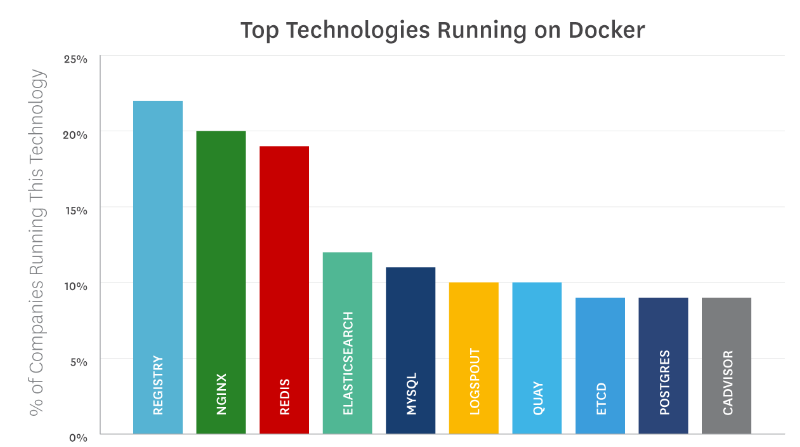
\includegraphics[width=15cm, height=9cm, scale=0.3]{docker-adoption.png}
	Quelle: https://www.datadoghq.com/docker-adoption/
\end{figure}
Betrachtet man Abbildung 3.1 wird deutlich, dass gerade im Webservice Bereich in Verbindung mit BigData Anwendungen, Docker am stärksten eingesetzt wird.
Um jedoch eine Vorstellung des Umfangs zu bekommen in wieweit Container eingesetzt werden, hilft ein Zitat von Joe Beda, Software Entwickler bei Google, welcher im Jahre 2014 folgendes verkündete.
\begin{quote}
	\footnote[2]{Vgl. https://speakerdeck.com/jbeda/containers-at-scale}
	"`\textit{Everything at Google runs in a Container}"\\
	"`\textit{We start over 2 billion containers per week.}"
\end{quote}
Dies machte nicht nur deutlich wie relevant diese Technologe ist, sondern zeugte auch von einer enormen Stabilität und Reife.\\
\\
Anwendungsbereiche, welche Docker bereits im Produktiveinsatz nutzen, beschränken sich jedoch nicht nur auf große Cloud Dienstleister.
Gerade im Bereich der Software Entwicklung beginnen viele Teams Docker für sich zu entdecken um Probleme und Barrieren bei DevOps zu überwinden.
Die Gründe dafür sind die besser Gewaltenteilung zwischen Entwicklern und Administratoren.
Es ist hierdurch möglich, dass ein Entwickler kontrollieren kann, was in einem Container geschieht ohne in einen Konflikt mit einem Administrator zu gelangen, welcher für die darunterliegende Infrastruktur zuständig ist. 
Zusätzlich ist es möglich innerhalb kürzester Zeit unterschiedliche Umgebungen und Tools für ein Team zur Verfügung zu stellen.
Ein weiterer sehr relevanter Punkt, ist das entwickeln und testen an einem Produktivsystem. Momentan durchläuft ein Software Projekt meist viele Instanzen und Umgebungen, bis schlussendlich das Produkt an den Kunden ausgeliefert wird. Durch den Einsatz von Docker kann dieser Workflow enorm verkürzt werden.\\
\\
Es bleibt abzuwarten welche weiteren Anwendungsbereiche, sich durch die Weiterentwicklung der Container Virtualisierung, zusätzlich öffnen werden.

\section{Tools}
Docker versucht zwar ein möglich vollständiges Framework zu erschaffen, besitzt jedoch noch einige Lücken und Probleme, welche momentan durch zusätzliche Tools gelöst werden.
Dabei treten auch immer mehr Drittanbieter in den Wettstreit, neue Services rund um die Container Virtualisierung anzubieten.\\
\\
Im folgenden sollen vier Tools vorgestellt werden, welche das Problem der Verwaltung und Orchestration angehen.
Diese können der Reihenfolge nach aufeinander aufsetzen und sich gegenseitig ergänzen.

\subsection{Docker Machine}
Da im Cloud und Big Data Umfeld, allgemein mit vielen verteilten Clustern gearbeitet wird, ist eine Manuelle Installation von Host Systemen sehr unpraktikabel.\\
\\
Wie viele andere Frameworks in diesem Bereich, bietet auch Docker, die Möglichkeit Host Systeme über eine zentrale Stelle automatisiert zu bespielen.
Hierzu wird das Tool Docker Machine benutzt.
Dieses kann dann über einen einzigen Befehl auf allen definierten Host Systemen ein Image aufspielen.
Dazu wird, wie in Abbildung 3.2 zu sehen, ein aktuelles ISO-Image der passenden Distribution geladen und auf dem Host System installiert.
Zusätzlich wird die Docker Engine wie auch passende SSL Zertifikate erzeugt und eine SSH Verbindung aufgebaut. 
Danach steht das System zum Einsatz bereit.\\
\\
Diese Vorgehensweise kann in Kombination mit Docker Compose und Docker Swarm dazu genutzt werden, innerhalb kürzester Zeit ein komplettes Cluster in Betrieb zu nehmen.\\
\\
Docker unterstützt hierbei unzählige Anbieter:\\
\\
\textit{AWS, Digital Ocean, Google Cloud Platform, IBM Softlayer, Microsoft Azure und Hyper-V, OpenStack, Rackspace, VirtualBox, VMware Fusion, vCloud Air und vSphere}\\
\\
\begin{figure}
	\centering
	\caption{Docker-Machine}
	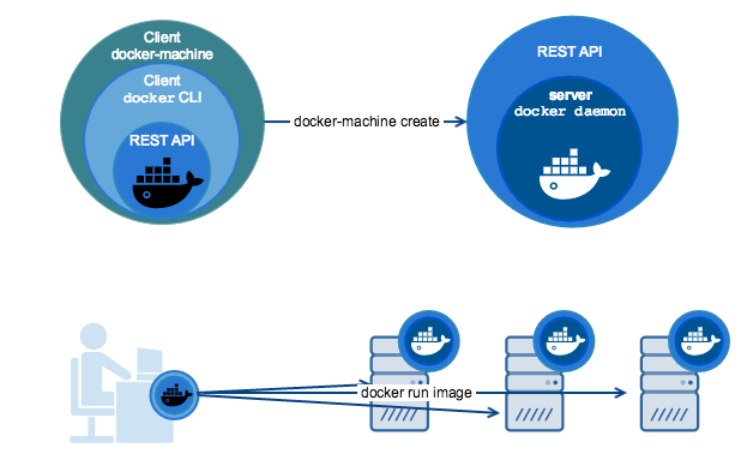
\includegraphics[width=15cm, height=9cm, scale=0.3]{docker-machine.png}
	Quelle: https://docs.docker.com/machine/overview/
\end{figure}
\subsection{Docker Compose}
Der Einsatz von großen Mengen an Containern erzeugt ganz natürlich einen enormen Verwaltungs- und Konfigurationsaufwand.
Aus diesem Grund entstanden sehr schnell unterschiedliche Lösungsansätze, um große Teile davon zu automatisieren.\\
\\
Selbst kleine Web Projekte bestehen aus unterschiedlichen Services welche zusammen arbeiten müssen um eine lauffähige Applikation zu kreieren.
Hierzu gehören z.B. Datenbanken, Authentifizierungservices, Web Server und Load Balancer um nur wenige zu nennen.
Um den Betrieb der Hauptapplikation, im falle von Problemen oder Änderungen, nicht vollständig zu gefährden, empfiehlt es sich für jeden Service eine isolierte Umgebung zu schaffen.
Dies führt jedoch in der Praxis sehr schnell zu Verwirrung in Kombination mit aufwändigen Dokumentationen und Aufstockung von administrativem Personal.\\
\\
Ein Tool welches einen Teil dieser Problematik löst ist Docker Compose.
Beim Einsatz von Compose, wird die komplette Applikationsumgebung in einer Konfigurationsdatei definiert und kann dann mit nur einem Befehl in Betrieb genommen werden.
Ausserdem wird dem Pool an Containern zusätzlich ein Projekt Name zugewiesen, um ihn von möglichen weiteren Instanzen abzugrenzen.
Dieser Container Zusammenschluss ist dann über einen einzigartigen Namen ansprechbar.\\
\\
Im Produktiveinsatz hat dies mehrere Vorteile:
\begin{itemize}
\item Mehrere Webapplikation welche aus verschiedenen Containern bestehen, können parallel ausgeführt werden ohne miteinander in Konflikt zu geraten.
\item Die Konfigurationsdatei dient zusätzlich als Dokumentation.
\item Durch die schnelle Inbetriebnahme werden automatisierte Tests stark vereinfacht und beschleunigt.
\end{itemize}
Docker Compose besitzt jedoch den Nachteil, dass es nur auf einem Host System funktioniert und somit alleine nicht für große und verteilte Applikationen einsetzbar ist.  
\subsection{Docker Swarm}

Um den Nachteil von Docker Compose aufzulösen, entstand im laufe der Entwicklung des Docker Frameworks, eine Native Cluster Lösung.\\
\\
Bekannt unter dem Namen Docker Swarm, sorgt dieses Tool dafür (siehe Abbildung 3.3), unterschiedliche Host Systeme zu einem virtuellen Docker Host zu bündeln.
Zusätzlich sorgt es dafür, dass wichtige Funktionalitäten, wie hohe Verfügbarkeit und Ausfallsicherheit, im Produktiveinsatz verfügbar sind.
Dabei ist die Inbetriebnahme nicht weiter komplex und auch durch Drittanbieter-Tools umsetzbar.\\
\begin{figure}
	\centering
	\caption{docker-swarm}
	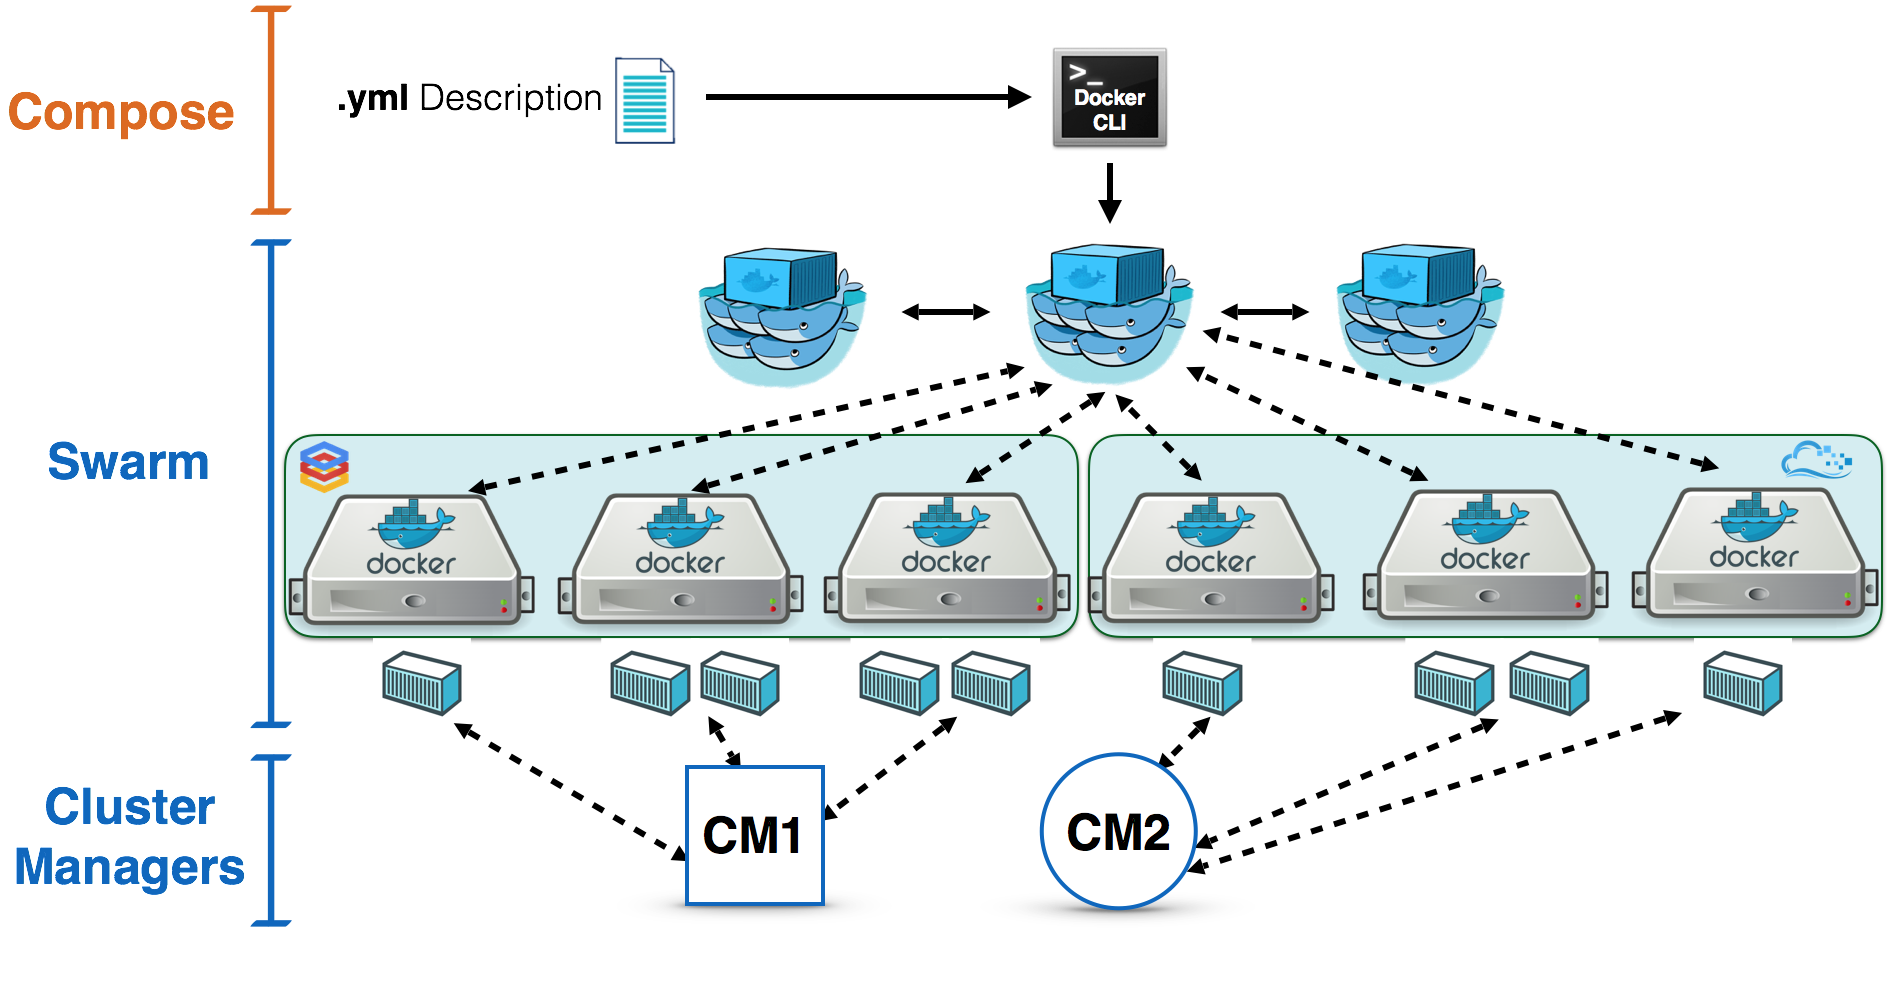
\includegraphics[width=15cm, height=9cm, scale=0.3]{docker-swarm.png}
	Quelle: https://blog.docker.com/2015/11/deploy-manage-cluster-docker-swarm/
\end{figure}
\\
Dies wird durch den kompletten Support der Docker API möglich und folgt auch hier folgendem Leitsatz:

\begin{quote}
	\footnote[1]{Vgl. https://docs.docker.com/v1.6/swarm/}
	"`\textit{"batteries included but removable"}
\end{quote}
Seit Version 1.12.0 ist Swarm ein fester Bestandteil der Docker Engine.\cite{swarm}
\subsection{Kubernetes}
Bevor Docker überhaupt veröffentlicht wurde, experimentierte Google schon seit langem mit LXC- Containern und entwarf hierfür eine Cluster Lösung, um die stetig wachsende Container-Landschaft unter Kontrolle zu halten.
Mit der steigenden Beliebtheit von Docker stellte Google schließlich sein System Kubernetes als Open Source Lösung zur Verfügung.
Die Idee der Bündelung von Containern unterscheidet sich hierbei kaum zwischen Docker Swarm und Kubernetes, jedoch wurde diese auf unterschiedlichen Wegen umgesetzt.
Zusätzlich kann Kubernetes auf einen Erfahrungsschatz von über 15 Jahren im produktiven Umfeld zurück greifen.\\
\\
Einige Funktionen sind z.B. :

\begin{itemize}
	\item Einem Container Bündel (auch Pod genannt) können klare CPU und RAM vorgaben erteilt werden, wodurch automatisiert der optimale Knoten ausgewählt werden kann.
	\item Kubernetes entscheidet automatisiert wie viele Pods gerade aktiv sein müssen.
	\item Es ist möglich einen Rollout im laufenden Betrieb durchzuführen ohne den Betrieb hierfür zu unterbrechen. Sollte dabei ein Problem auftauchen, wird automatisch ein Rollback durchgeführt.
	\item Support für unterschiedlichste Speichermöglichkeiten. Egal ob Lokal oder von einem Cloud Dienstleister.
	\item Automatisierte Bereinigung von abgestürzten Containern und Knotenpunkten.
\end{itemize}
Obwohl Docker Swarm und Kubernetes versuchen dieselben Probleme zu lösen, so sind die Lösungsansätze doch sehr verschieden und können je nach Anwendungsfall besser oder aber auch schlechter sein.

\section{Wieso gerade Docker ?}
Wie anfangs betont ist die Geschichte der Container Virtualisierung weitaus älter und umfangreicher als man dies vermuten möchte.
So stellt sich also die Frage, warum gerade durch die Veröffentlichung von Docker diese Art der Virtualisierung so enorm an popularität gewonnen hat.
Warum konnten frühere Formen wie LXC oder OpenVZ nicht denselben Erfolg erreichen.\\
\\
Docker kam zur richtigen Zeit und brachte dabei Funktionalitäten mit sich, welche frühere Umsetzungen nicht besasen.
Dazu gehörte an erster Stelle, dass der Ansatz von Docker eine einfachere und sichere Verbreitung von Containern erlaubt.
Mit der Veröffentlichung von libcontainer und der Partnerschafft zu vielen zentralen IT Firmen, machte Docker den Weg frei für eine Standardisierung im Container Umfeld, welche auf wirtschaftlicher Ebene von enormer Wichtigkeit ist.
Wie Github eine zentrale Anlaufstelle für das collaborative Arbeiten und verteilen von Softwareprojekten ist, so gibt DockerHub der Community eine Plattform über welche Container zentral verwaltet und gewartet werden.
Dies führt zu einer fülle von Diensten welche innerhalb von wenigen Sekunden geladen und genutzt werden können.\\
Mit weiteren Projekten wie Docker Swarm, Docker Compose, Docker Registry oder auch Docker Toolbox wird dem Nutzer ein großes und schon jetzt, sehr ausgereiftes Reportoir and Tools geboten, welche den Einsatz von Containern immer komfortabler gestalten.\\
\\
Firmen wie z.B. Red Hat versuchen zwar selbst neue Frameworks für die Container Virtualisierung auf den Markt zu bringen können jedoch nicht auf eine solch umfangreiche Community zurück greifen.

\chapter{Fazit - Ausblick} % (fold)
\label{sec:fazit}

Docker ist ein Werkzeug, welches optimal in eine Zeit von Microservices, Big Data und Cloud Computing passt.
Es unterstützt durch sein nahezu vollständiges Framework einen sehr reibungslosen Arbeitsablauf und bringt dadurch eine gewisse Stabilität in eine ungewisse Zeit.
Unterstützt durch Firmen wie Cisco, Google, Huawei, IBM, Microsoft und Red Hat kann ganz klar gesagt werden, das Docker sicherlich nicht nur eine Moderscheinung ist, sondern uns noch eine weile begleiten wird.\\
\\
Untersuchungen von Datadog über das verhalten von Firmen im Bezug auf den Einsatz von Containern unterstützen diese Behauptung.
Im letzten Jahr stieg hierbei der Einsatz um 30\% im Vergleich zum Vorjahr wobei es erstaunlich ist, dass gerade große Firmen sehr schnell den Einsatz von Docker umsetzen.
Auch ist interessant, dass der meistgenannte Grund, warum Container eingesetzt werden die erhöhte Effizienz in der Entwicklung ist.
So kann sich auch Docker sicherlich bald unter den Standard Tools der Entwicklungswerkzeuge einfinden.\\
\\





https://clusterhq.com/2016/06/16/container-survey/
https://www.datadoghq.com/docker-adoption/

% chapter fazit (end)

\appendix
\begin{thebibliography}{99}
\raggedright
%%% Printquellen zuerst
%%% Beispiel
\bibitem{Th11} Manuel René Theisen:
 \emph{Wissenschaftliches Arbeiten: Technik -- Methodik -- Form};
 15.~Auflage; Vahlen; München 2011;
 ISBN 978-3-8006-3830-7

%%% Internetquellen: Beispiel
\bibitem{jenkins} \emph{Jenkins};
 \url{https://jenkins.io/};
 abgerufen am 02.12.2016
 
\bibitem{dockerWhat} \emph{Docker};
 \url{https://www.docker.com/what-docker};
 abgerufen am 02.12.2016
 
 \bibitem{swarm} \emph{Docker Swarm};
 \url{https://docs.docker.com/engine/swarm/};
 abgerufen am 02.12.2016
 
 


 
 
 
 
 
 
\end{thebibliography}
\end{document}

